\style{mb}


\section{Les fractions avec \mb}

%   logo mb dans la table des matières


% style de page micro:bit
%\pagestyle{mb}

\subsection{Description}

\subsubsection{Objectif}

\begin{formule}
Le but de ce projet est :
\begin{description}
    \item [cycle 4] 
        Utiliser diverses représentations d’un même nombre ; passer d’une représentation à une autre.\\
        Comparer, ranger, encadrer des nombres rationnels.
    \item [\textsc{CAP}] 
        Comparer, additionner, soustraire, multiplier et diviser les nombres en écriture fractionnaire dans des situations simples.
\end{description}

\end{formule}

\subsubsection{Intérêt}
Les fractions posent en général des difficultés aux élèves et la majorité font des blocages hérités des années antérieures. Le risque de démobilisation est grand et l'usage d'un objet connecté permet de dédramatiser la séance.

\begin{description}
    \item [Aspect ludique] L'usage de l'affichage LED du micro:bit rend l'activité ludique. Les élèves sont pour la plupart attirés par le côté simple et sympathique de l'écran, ce qui les poussent à réfléchir et s'investir.    
    \item [Proportions] Afficher une image conforme à une contrainte est un problème concret qui permet de mieux matérialiser un calcul de proportion, par rapport à un énoncé classique (type statistiques). En évaluation, il y a plus de réponses justes quand la question repose sur un affichage d'image que sur une situation plus habituelle (point vérifié en classe).
    \item [Plusieurs de méthodes de résolutions] Il y a de nombreuses façons d'arriver aux solutions. Par exemple pour éclairer $\frac{2}{5}$ des LED, on peut d'abord \emph{faire des paquets} de 5, en allumer 2 puis recommencer ; soit éclairer \emph{2 colonnes sur les 5} existantes.
\end{description}


\subsubsection{Matériel}
\begin{itemize}
    \item 1 $\times$ \matosMb \emph{(facultatif car le simulateur peut suffire, même si on perd un peu sur l'aspect ludique.)}
    \item 1 $\times$ accès internet : IDE programmation par bloc \url{http://makecode.microbit.org/}
\end{itemize}



%
% activité de niveau 
%
\newpage
\subsection{Écrire une fraction}
\subsubsection{Activité élève}

% commande perso \CARTOUCHE
%   5 paramètres : 
%       * durée
%       * public
%       * travail en maths
%       * travail en sciences
%       * travail en algo
\cartouche
{0,5 h}
{Cycle 4 ; CAP}
{représentation d'un nombre ; fraction}
{}
{}




%
%   ELEVE
%

\begin{wrapfigure}[1]{r}{1.5cm}
    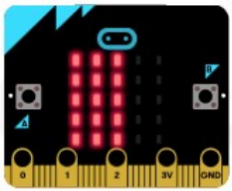
\includegraphics[width=\linewidth]{res/mb-fraction-mini.png}
\end{wrapfigure}




\begin{eleve}    
    \texttt{Écrire la proportion de LED allumée sur chaque micro:bit}
    
    \centerline{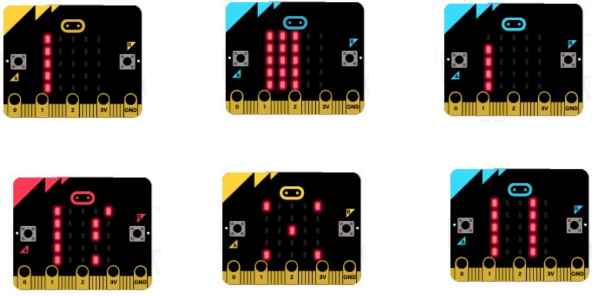
\includegraphics[width=0.75\linewidth]{res/mb-fraction.png}}
\end{eleve}

%
%   PROF
%

\subsubsection{Notes pour l'enseignant}

Attendus:

\begin{itemize}
    \item Les élèves écrivent les fractions correspondant pour chaque appareil.
    \item Lorsque c’est possible, on écrit la fraction sous différentes formes : $\frac {1}{5}$ ou $\frac{5}{25}$.
    \item On écrit alors les conditions d’égalité de deux fractions.
\end{itemize}

\begin{remarque}
    Prolongement  possibles :
    \begin{itemize}
        \item Répondre par une phrase : \emph{il y a 5 LED allumées sur un total de 25}.
        \item Pour chaque cas, indiquer la proportion de LED \emph{éteintes}.
    \end{itemize}
\end{remarque}


%
% activité de niveau 
%
\newpage
\subsection{Afficher une fraction}
\subsubsection{Activité élève}

% commande perso \CARTOUCHE
%   5 paramètres : 
%       * durée
%       * public
%       * travail en maths
%       * travail en sciences
%       * travail en algo
\cartouche{0,5 h}{Cycle 4 ; CAP}{représentation d'un nombre ; fraction}{}{affichage}

%
%   ELEVE
%
\begin{wrapfigure}[4]{r}{3cm}
    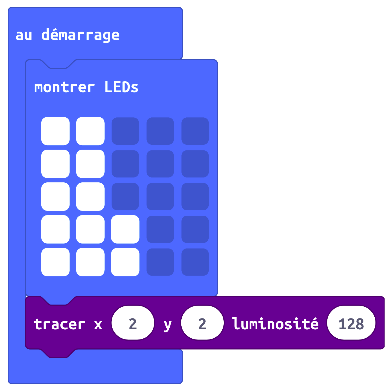
\includegraphics[width=\linewidth]{res/mb-fraction2.png}
\end{wrapfigure}

\begin{eleve}    
    \texttt{Représenter les fractions suivantes avec les LED du micro:bit}
    $$
    \frac{1}{2} \quad ; \quad \frac{32}{100}
    $$
\end{eleve}

%
%   PROF
%
\subsubsection{Notes pour l'enseignant}

Attendus :

\begin{itemize}
    \item Les élèves constatent qu’il n’est pas possible d’afficher un demi, on peut alors leur suggérer d’afficher la 13ème led en alternance ou de lui réduire la luminosité.
    \item Les élèves doivent simplifier la deuxième fraction pour afficher, on peut alors faire le lien avec les pourcentages
\end{itemize}


%
% activité de niveau 
%
\newpage
\subsection{Somme de fractions}
\subsubsection{Activité élève}

% commande perso \CARTOUCHE
%   5 paramètres : 
%       * durée
%       * public
%       * travail en maths
%       * travail en sciences
%       * travail en algo
\cartouche{0,5 h}{Cycle 4 ; CAP}{représentation d'un nombre ; fraction}{}{affichage}

%
%   ELEVE
%
\begin{wrapfigure}[4]{r}{3cm}
    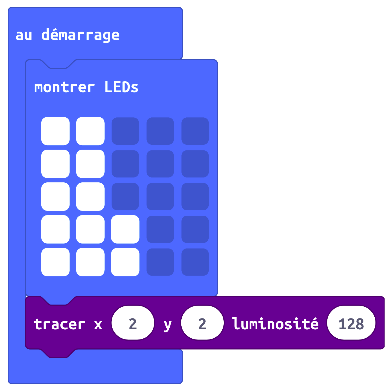
\includegraphics[width=\linewidth]{res/mb-fraction2.png}
\end{wrapfigure}

\begin{eleve}    
    \texttt{Représenter les fractions suivantes avec les LED du \mb :}
    $$
    \frac{2}{5} + \frac{3}{25} \quad ; \quad \frac{23}{25}
    $$
\end{eleve}

%
%   PROF
%
\subsubsection{Notes pour l'enseignant}

\begin{remarque}
Plusieurs raisonnements sont à construire :
\begin{itemize}
    \item créer des paquets de 5 et prendre à chaque fois 2 éléments 
    \item diviser le tout en 5 paquets et en prendre 2
    
\end{itemize}
    
\end{remarque}